% !TeX spellcheck = en_GB
\chapter{\IfLanguageName{dutch}{Stand van zaken}{State of the art}}
\label{ch:stand-van-zaken}
In this chapter, the state of affairs will be examined. As mentioned in the introduction, this part of the bachelor's thesis will be used to get an in-depth understanding of the four key themes that incorporate the changes in Windows Server 2019. First, a basic understanding of what those four key themes are will be established. Afterwards, their implementation in the latest version of the \acrshort{os} will be looked into.

\section{Hybrid cloud}
Hybrid Cloud is a topic that has gained more momentum over the past years. For organizations, this makes it a consistent topic of interest and makes it a natural choice as one of the four keystone themes in Windows Server 2019.\autocite{MWST2018} With this in mind, the Hybrid Cloud will be discussed as an essential part of the bachelor's thesis. It is especially beneficial to know the advantages that it has to offer to Windows Server since the latest version. How these new and improved features enhance workflow and how they can be leveraged by organizations, in particular, Delaware. To start with, the different types of clouds will be discussed in the following subsection, as a start.

\subsection{Types of cloud solutions}
The National Institute of Standards and Technology differentiates four types of clouds\autocite{Mell2011}:
\begin{itemize}
	\item Private Cloud
	\item Community Cloud
	\item Public Cloud
	\item Hybrid Cloud
\end{itemize}	
It is important to keep in mind that virtualization and cloud computing are two different technologies. While virtualization detaches computing environments from their physical infrastructure through software, cloud computing is a service that delivers computing resources on demand through a network.\autocite{Naeem2016}

\subsubsection{Private cloud}
A private cloud is an internal infrastructure in the cloud that is designated for use by a single organization. It can, however, consist of multiple clients, provided those are in the same organization. It is only accessible inside a private internal network or over the internet for a selected amount of users. Private clouds cannot be accessed by the public. They can also be known by other names such as internal or corporate cloud. Their main advantage is the higher level of security and privacy, which is offered through the use of in-house hosted infrastructure and additional company firewalls. The biggest disadvantage that comes with this added layer of security is the responsibility that is given to the \acrshort{it} team who manages the infrastructure that supports the private cloud. This means, on top of the additional infrastructure costs, that they require the same amount of man-hours that comes with the management of a traditional data centre. Keep in mind that in-house does not necessarily mean on-premise.
\\
Still, the private cloud holds a great benefit compared to long-standing methods. As reported by IBM, an organization saved more than \$1.5 billion by reducing its number of data centres from 115 to 5. This was a direct result of the implementation of a private cloud.\autocite{Hofmann2010} 


\subsubsection{Community cloud}
When several organizations collaborate to meet the requirements that are demanded of the \acrshort{it} infrastructure, they are operating under a community cloud. This means that it can be managed in-house or by a third-party organization operating inside the same community. This form of operation tackles one of the main problems of a private cloud. It shares the costs over multiple organizations, thus greatly reducing it. Since they are operating inside the same community, they share the same concerns and will be subjected to the same requirements that can be imposed by a governing instance. 
However, this advantage over private clouds comes at a cost. This reduction in cost as a result of sharing the infrastructure results in a devaluation of security. Meaning that it is a viable alternative to organizations that have some security concerns with the usage of a public cloud, but are willing to make some sacrifices in favour of a cost reduction. 
\\
An example of this is described in an article by \textcite{Yao2014}. The research shows how small hospitals in China, not all of which can provide their own infrastructure, could utilize a community cloud. These grass-roots healthcare institutions, that all operate within the same community, can share the cost and management of the cloud to provide an attractive hospital information solution to improve their service without the extensive cost nor the need for additional security concerns regarding confidential information in patient files.

\subsubsection{Public cloud}
Amazon Web Services, Oracle Cloud and Microsoft Azure are some examples of public clouds. Most of these solutions are offered by corporations who manage and operate their data centres and provide access to their cloud via the internet. Thus eliminating the cost that is associated with the management and responsibility of a private cloud and so significantly reduces the cost in comparable use cases. Public clouds also provide the possibility for effortless scalability and flexibility in comparison with private clouds, where the required hardware for scaling needs to be available in-house. This makes the public cloud ideal for temporary solutions and fast-growing organizations.
\\
\textcite{Singh2012} concluded, in a comparison between the cost and security of private and public clouds over three years, that although security can be a real concern in the usage of public cloud it should not be ruled out immediately without fully analysing the requirements of an organization. Keeping in mind the major investment that comes with the usage and implementation of a private cloud.  
The different obstacles that securing a public cloud have also been addressed by \textcite{Ren2012}, in which there is a call for additional research about the subject to fully take advantage of the breakthrough that cloud computing is. 

\subsubsection{Hybrid cloud}
A hybrid cloud aims to be the solution for every kind of organization. It combines a higher level of security and privacy that is offered by a private cloud solution with easy scalability and flexibility that comes paired with the public cloud. A hybrid cloud is a contraption of two, or more, of the previously mentioned types. This translates to a combination of private and public cloud solutions in most use cases. As described in the book by \textcite{Sarna2010}, hybrid clouds enable large organizations to move their less sensitive information, like \acrfull{hr}, to the cloud. Thanks to the advantages of hybrid cloud their sensitive data, such as classified information about customers or the organization, can remain in-house on private clouds or even on-premise for an additional layer of security. The connection between the public and private cloud of the hybrid cloud is generally accomplished through a secure connection, for example, \acrfull{vpn}.

\subsection{Hybrid cloud in Windows Server 2019}
\label{hybrid-cloud-windows-server-2019}
As mentioned before, Microsoft offers a hybrid cloud solution that combines the private cloud of an organization with Microsoft Azure, its public cloud solution. Microsoft Azure is offered from 34 sets of data centres all over the world. Microsoft is confident that clients who are running the latest version of Windows Server, and the associated software, can have a hybrid cloud set-up almost instantly. This through the usage of a new feature that significantly simplified the management of the hybrid cloud. Nowadays this feature is known as Windows Admin Center, previously as Project Honolulu. Windows Admin Center was built with a hybrid cloud, and \acrshort{hci}, in mind. This tool, built to manage Windows Server and Windows 10, is optimized for use within Windows Server 2019. This constitutes an additional argument for a migration to the latest version. The entire step-by-step plan for Windows Admin Center Azure Integration is given in Appendix \ref{WACAzure}. Once this has been completed the following features \autocite{Washburn2018} can be leveraged through Windows Admin Center:
\begin{description}
\item [Azure Active Directory authentication] Provides access to Azure Active Directory which adds a layer of security and ease of management and scalability.
\item [Manage Azure IaaS virtual machines] Manage on-premise \acrshort{vm}s as well as Azure \acrshort{vm}s.
\item [Azure Site Recovery] Provides back-up and recovery services for business continuity and disaster recovery.
\item [Azure Update Management] An Azure Automation solution to manage updates and patches for on-premise, external hosted or Azure \acrshort{vm}s.
\item [Azure Network Adapter] Securely connect the local computer to Azure Virtual Network.
\end{description}

\clearpage

\section{Security}
With more than 53.000 reported incidents and 2.216 confirmed data breaches \autocite{Verizon2018}, security has become an essential part of \acrshort{it}. The importance of security directly translates into Windows Server 2019 through various parts of the \acrshort{os} that have either been reviewed to make them more resilient and accessible or new features which have been added to further improve security. In the following section all the major elements will be discussed, distributed among three subsections:
\begin{itemize}
	\item Windows Defender \acrfull{atp}
	\item Security with \acrfull{sdn}
	\item Shielded Virtual Machines (VM)
\end{itemize}

\subsection{\acrfull{wdatp}}
In a research study done by \textcite{Musto2017} \acrshort{wdatp} was scrutinized. When the endpoint security solution is implemented in Windows Server 2019, it will require additional licensing. Still, the efficiency with which it tackles security problems resulted in a 53\% \acrfull{roi}. The research reported that \acrshort{wdatp} reduced the risk of a breach by 40\%. It even enabled them to identify threats faster and resolve them in a more efficient fashion. In conclusion, the replacement of previous solutions with \acrshort{wdatp} reduced costs and made security teams more efficient. With the advent of Windows Server 2019, additional features have been added to \acrshort{wdatp} to ensure the safety of organizations in the years to come. The different components of \acrshort{wdatp} are described in Figure \ref{fig:WDATPT2018}. Those will not be individually reviewed here as this subject of endpoint security alone offers enough content for another bachelor's thesis.
\begin{figure}[hbt!]
	\centering
	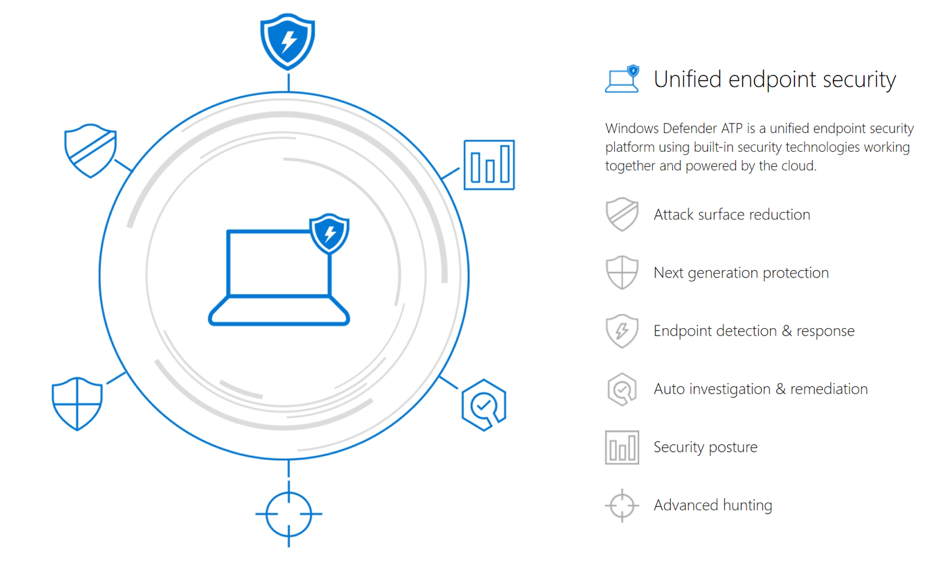
\includegraphics[width=\textwidth,height=6cm,keepaspectratio=true]{img/StandVanZaken/WDATP.png}
	\caption[Components of \acrshort{wdatp}]{The different components of \acrfull{wdatp}. \autocite{Aslaner2018}}
	\label{fig:WDATPT2018}
\end{figure}

\subsection{Security with \acrshort{sdn}}
\label{encrypted-networks}
\label{sdn}
As described by \textcite{Shin2016}, \acrshort{sdn} is a state-of-the-art technology that enables developers to design advanced networks effortlessly. In Windows Server 2019 there have been new developments in this field. These can be boiled down to four features: 
\begin{itemize}
	\item Encrypted networks
	\item Firewall auditing
	\item Virtual network peering
	\item Egress metering
\end{itemize} 
The discussion of these will be kept constrained.
\subsubsection{Encrypted networks}
Encrypted networks, or more specifically virtual encrypted networks, enable the encryption of network traffic between different \acrshort{vm}s. By the use of \acrfull{dtls}. \acrshort{dtls} was built as close to \acrfull{tls} as possible, which makes it ideal at securing connections. However, for the connection between \acrshort{vm}s \acrshort{dtls} is preferred, since these connections are delay sensitive.\autocite{Modadugu2004}

\subsubsection{Firewall auditing}
One of the new features in Windows Server 2019 is \acrshort{sdn} Firewall auditing. This means that the administrator has the opportunity to examine if every part of the Firewall is as secure as initially thought. When this feature is enabled every data stream that gets processed by the \acrshort{sdn} firewall, gets recorded. The logs can be used in troubleshooting or archived for analysis. These can also be processed by tools such as Power BI.

\subsubsection{Virtual network peering}
Virtual network peering allows administrators to combine two individual virtual networks. A coherent connection is made that represents itself as an individual one. This means the connection between both networks can be routed through the infrastructure backbone. This in term means that there is no need for a public gateway. Providing a more secure connection, while no additional downtime is accumulated when peering the networks.

\subsubsection{Egress metering}
Egress metering for \acrshort{sdn} enables an administrator to monitor the consumption of outgoing connections. Windows Server 2019 also makes a distinction between traffic that leaves the virtual network and the data centre, in comparison to traffic that stays within the data centre. 

\subsection{Shielded Virtual Machines}
One of the requirements to run a Shielded \acrshort{vm} is a \acrfull{hgs}. Since Windows Server 2019 it is possible to run Shielded \acrshort{vm}s on machines with an irregular connection to the \acrshort{hgs}. This can be done by leveraging the following two new features:

\begin{description}
	\item[Fallback \acrshort{hgs}] Provide a redundant connection in case the primary \acrshort{hgs} can not be reached.
	\item[Offline Mode] Once a shielded \acrshort{vm} has been setup it can be started up seeing that the security configuration remains unchanged.
\end{description}

Another new feature is the addition of support for Ubuntu, Red Hat Enterprise Linux and SUSE Linux Enterprise Servers inside Shielded \acrshort{vm}s. 

\clearpage

\section{Application platform}
An application platform is an essential part of \acrshort{it} operations. It provides services to applications so that these can run fluently. A modern application platform is extensive, it provides an array of services to a variety of applications. According to a paper by \textcite{Chappell2011}, there are five categories of services offered by an application platform:
\begin{itemize}
	\item \acrshort{os}
	\item Execution services
	\item Data services
	\item Cloud services
	\item Development tool
\end{itemize}
These five categories are not necessary for every application but should be offered in a modern application platform nonetheless.
There have been major improvements in this area with the arrival of Windows Server 2019.\autocite{Gerend2018} 
\\
In the following paragraphs, these will be discussed and analysed to a certain extent.

\subsection*{Linux containers on Windows}
Since Windows Server 2019 it is now possible to run Linux containers on the same container host, utilizing the same Docker daemon. This is an important addition knowing that only 3.23\% of all Apache servers runs on Windows. \autocite{SecuritySpace2019}
\subsection*{Building Support for Kubernetes}
Kubernetes is a software solution designed to oversee containers. It is a management environment for network, computing and data infrastructure. With Windows Server 2019 this has been further developed inside the \acrshort{os}. For now, there has been a great improvement in container networking, but as new versions of Kubernetes are rolled out additional features will be added with updates through semi-annual channel releases.
\subsection*{Container improvements}
Containers as a whole have also been improved. There is better support for Windows Authentication inside containers as well as improved application compatibility for the existing Windows Server Core image. Other base images have also been reduced in size and overall performance has been improved.
\subsection*{Encrypted Networks}
This has been discussed in Subsection \ref{encrypted-networks}.
\subsection*{Network performance improvements for virtual workloads}
To increase throughput in virtual machines two new features have been introduced:
\begin{itemize}
	\item \acrfull{rsc} in the vSwitch
	\item \acrfull{dvmmq} and \acrfull{vrss}
\end{itemize}
\subsection*{\acrfull{ledbat}}
\acrshort{ledbat} is a delay-based congestion control algorithm that designates bandwidth to users and applications, but still using the totality of the network when it is available. \autocite{Shalunov2012}
This makes it interesting for deploying large updates in large-scale \acrshort{it} environments without impacting users.
\subsection*{High performance \acrshort{sdn} gateways}
The throughput of existing \acrshort{sdn} gateways has been improved. This by improving the throughput for \acrfull{ipsec} and \acrfull{gre} connections. Additionally, the required CPU utilization has been lowered.
\subsection*{Persistent Memory support for Hyper-V VMs}
Storage-class memory, or also known as persistent memory, improves latency and delivers a high throughput. To leverage this in \acrshort{vm}s, the two can now be directly connected.
\subsection*{New Deployment UI and Windows Admin Center extension for \acrshort{sdn}}
As already mentioned before , in Subsection \ref{hybrid-cloud-windows-server-2019}, Windows Admin Center also implements certain features to make managing \acrshort{sdn} easier. The extension that provides this is only available in an \acrshort{hci}.

\clearpage

\section{\acrfull{hci}}
Estimates made in a report by \textcite{Gantz2012}, show that the digital universe will consist of 50.000 Exabytes by the year 2020. This means that the infrastructure needs to be able to store these vast amounts of data. The static and inflexible way of storing data needs to become dynamic and agile to conform to modern standards. This can be achieved through a \acrfull{sddc}. It was developed to further leverage the success that is virtualization. An \acrshort{sddc} can be achieved in multiple ways but the most efficient and popular method is through \acrshort{hci}. It converges the compute, storage, networking and management components, as can be seen in Figure \ref{fig:HCI}, through software that is running on the hypervisor. In addition to the advantages that comes with \acrshort{hci}, they deliver strong support for the deployment of a hybrid cloud, one of the other key themes in Windows Server 2019. 
\acrshort{hci} reinvents how to store data through \acrshort{s2d}, which was one of the most anticipated features to be included in Windows Server 2019. This will be discussed below together with Hyper-V, \acrshort{sdn} and how these components can be managed through the Windows Admin Center. \autocite{Haag2016}
\begin{figure}[h]
	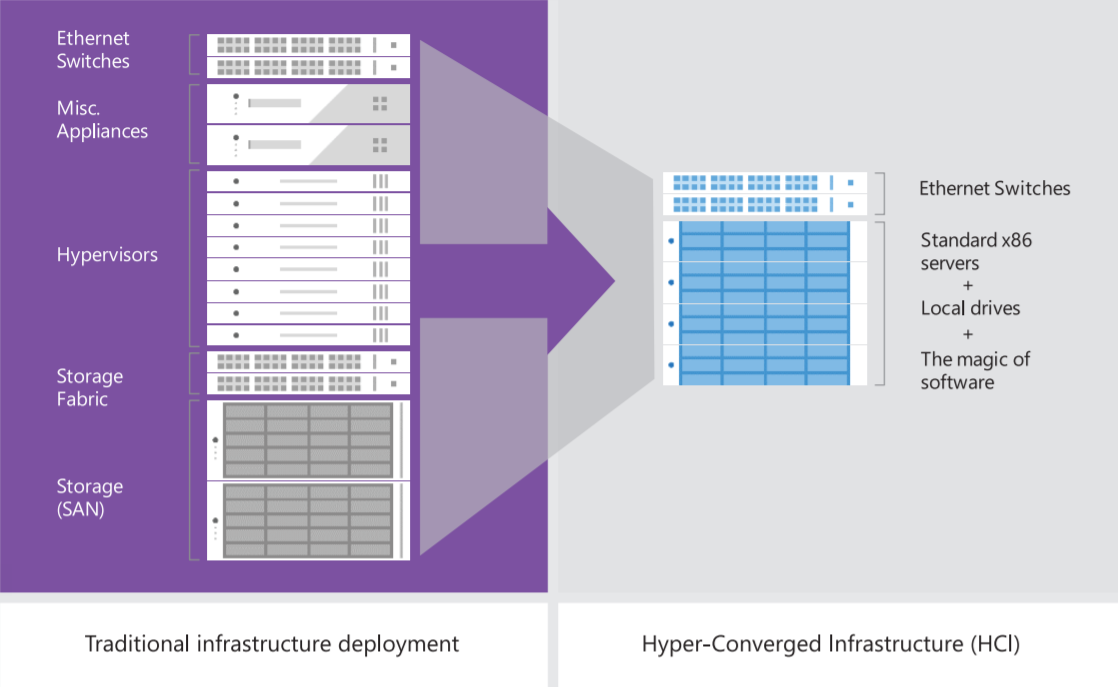
\includegraphics[width=0.8\linewidth]{img/StandVanZaken/HCI.png}
	\captionsetup{width=0.6\linewidth}
	\centering		
	\caption[\acrshort{hci}]{\acrfull{hci}}
	\scriptsize	
	Adapted from \cite{Woolslayer2018}
	\label{fig:HCI}
\end{figure}

\subsection{Hyper-V}
As mentioned in the introduction, an \acrshort{hci} requires a Hypervisor. In Windows Server, this is provided by Hyper-V. It can be used to virtualize compute, storage, networking and management components.  It does this by creating \acrshort{vm}s, that acts as an entire computer. They all run in their own isolated space, which translates in the ability to run multiple of these on a single hypervisor. The previously mentioned advantages also apply to Hyper-V. The provided services make room for a scalable and flexible infrastructure. To summarize, Hyper-V provides the Hypervisor that is an essential part of an \acrshort{hci}. \autocite{Short2016}
\subsection{\acrfull{s2d}}
Another vital component of \acrshort{hci} is \acrfull{sds}. In Windows Server, this is done through \acrshort{s2d}. This technology was developed to provide flexible and agile \acrshort{sds}. Some key benefits offered are simplicity, performant storage, fault tolerant and scalability. With Windows Server 2019 comes the largest update for \acrshort{s2d} since its introduction with Windows Server 2016. The licensing for this feature is also included in Windows Server 2019 Datacenter Edition, which means that for most clients, it will not involve an additional cost. \autocite{Gerend2018a}
\subsection{\acrshort{sdn}}
As previously mentioned in Subsection \ref{encrypted-networks}, \acrshort{sdn} gives form to the networking component of \acrshort{hci}. It provides \acrshort{it} administrators with the ability to design advanced networks effortlessly.
\subsection{Windows Admin Center}
Windows Admin Center is an all-in-one platform for local and remote server management. The key components of which it consists listed below, make it no surprise that the Windows Admin Center has been mentioned before. 
\begin{itemize}
	\item Core tools
	\item HCI Management
	\item Security
	\item Built for Hybrid
	\item Partner Ecosystem
\end{itemize}
It is Windows Server Management reimagined, with the input of costumers kept in high regard. It is the glue that joins all other components under one \acrfull{ui}. This tool is also the final part of our \acrshort{hci} environment, as it combines storage (\acrshort{s2d}), network (\acrshort{sdn}) and computing (Hyper-V) components under its management interface. 

\section{Conclusion}

Windows Server 2019 is a highly advanced \acrshort{os}. With the many new features it provides a smooth and manageable experience to administrators and \acrshort{it} professionals. The four key themes, that have been further developed to offer many improvements, have been thoroughly discussed in the previous sections and make it interesting to negotiate the migration regardless of its size. Furthermore, the extended support for Windows Server 2019 will be provided until 2029, this makes it a investment in the future of any organization. In the next chapter, the different methods for migrating the system will be discussed.
